\chapter{排序}\label{DS08}

\section{稳定性、内外排序与计数口径}\label{DS08-definition}

排序移动整条记录，以关键字确定次序。稳定排序保证相等关键字记录的原相对次序；用\(2_a、2_b\)追踪身份。稳定性为对全部合法输入的保证，单份无重复数据无法检验。

内部排序在处理期间全部记录驻内存；外部排序需分批交换内外存，主要计块I/O。比较次数、移动次数、趟数和辅助空间分别统计。

本章直接插入一趟处理一个新记录，希尔一趟处理一个增量的全部组，归并一趟处理全部相邻段。快排过程题按同一深度全部未定子区间各划分一次为一趟；程序若按单次划分计趟，以具体定义为准。

\section{直接插入与折半插入}\label{DS08-insertion}

直接插入保持有序前缀，将新值前所有严格大于它的值后移，插在旧相等值后，因而稳定。以下采用\texttt{A[\allowbreak{}1.\allowbreak{}.\allowbreak{}n]\allowbreak{}}、\texttt{A[\allowbreak{}0]\allowbreak{}}暂存兼哨兵，数组需\(n+1\)单元。

\par\smallskip\noindent\begin{minipage}{\linewidth}
\begin{codeblock}[language={C++}]
void InsertSort(int A[], int n) {
    int i,j;
    for (i=2; i<=n; ++i)
        if (A[i]<A[i-1]) {
            A[0]=A[i];
            for (j=i-1; A[0]<A[j]; --j)
                A[j+1]=A[j];
            A[j+1]=A[0];
        }
}
\end{codeblock}
\end{minipage}\par\smallskip

有序输入每趟只比较一次，最好\(\Theta(n)\)；逆序输入的有效记录后移数为\(n(n-1)/2\)（暂存与写回另计），平均、最坏\(\Theta(n^2)\)，空间\(O(1)\)。

折半插入在有序前缀中找第一个大于新值的位置，减少比较，搬移仍可能二次：

\par\smallskip\noindent\begin{minipage}{\linewidth}
\begin{codeblock}[language={C++}]
void BinaryInsertSort(int A[], int n) {
    int i,j,low,high,mid;
    for (i=2; i<=n; ++i) {
        A[0]=A[i];
        low=1; high=i-1;
        while (low<=high) {
            mid=(low+high)/2;
            if (A[mid]>A[0]) high=mid-1;
            else low=mid+1;
        }
        for (j=i-1; j>=high+1; --j) A[j+1]=A[j];
        A[high+1]=A[0];
    }
}
\end{codeblock}
\end{minipage}\par\smallskip

每趟均完整折半定位时，总比较\(\Theta(n\log n)\)，最好总时间亦\(\Theta(n\log n)\)；平均、最坏移动与总时间\(\Theta(n^2)\)。若先判断新值已不小于前缀末项并跳过定位，有序输入可线性，须按该实现重算。

\section{起泡与简单选择}\label{DS08-exchange-selection}

起泡仅交换相邻逆序，稳定；教材从后向前扫描，每趟把剩余最小记录送到前端。无交换即停，最好\(\Theta(n)\)，平均、最坏\(\Theta(n^2)\)，空间\(O(1)\)。

\par\smallskip\noindent\begin{minipage}{\linewidth}
\begin{codeblock}[language={C++}]
void BubbleSort(int A[], int n) {
    for (int i=0; i<n-1; ++i) {
        bool flag=false;
        for (int j=n-1; j>i; --j)
            if (A[j-1]>A[j]) {
                int temp=A[j-1];
                A[j-1]=A[j]; A[j]=temp;
                flag=true;
            }
        if (flag==false) return;
    }
}
\end{codeblock}
\end{minipage}\par\smallskip

简单选择每趟找未排序区最小记录，与首位交换。比较总数恒为\(n(n-1)/2\)，至多\(n-1\)次交换，所有情况时间\(\Theta(n^2)\)、空间\(O(1)\)。远距离交换可破坏稳定性：\(2_a,2_b,1\to1,2_b,2_a\)。

\par\smallskip\noindent\begin{minipage}{\linewidth}
\begin{codeblock}[language={C++}]
void SelectSort(int A[], int n) {
    for (int i=0; i<n-1; ++i) {
        int min=i;
        for (int j=i+1; j<n; ++j)
            if (A[j]<A[min]) min=j;
        if (min!=i) {
            int temp=A[i]; A[i]=A[min]; A[min]=temp;
        }
    }
}
\end{codeblock}
\end{minipage}\par\smallskip

\section{希尔排序}\label{DS08-shell}

每个正增量\(d\)将下标同余的记录作直接插入，完成后仅保证\(d\)间隔有序。增量逐步缩小，末增量必须1。希尔不稳定，复杂度依赖增量序列，空间通常\(O(1)\)。

\par\smallskip\noindent\begin{minipage}{\linewidth}
\begin{codeblock}[language={C++}]
void ShellSort(int A[], int n) {
    int d,i,j;
    for (d=n/2; d>=1; d=d/2)
        for (i=d+1; i<=n; ++i)
            if (A[i]<A[i-d]) {
                A[0]=A[i];
                for (j=i-d; j>0 && A[0]<A[j]; j-=d)
                    A[j+d]=A[j];
                A[j+d]=A[0];
            }
}
\end{codeblock}
\end{minipage}\par\smallskip

有效范围\texttt{A[\allowbreak{}1.\allowbreak{}.\allowbreak{}n]\allowbreak{}}，0号只暂存；并非每组均能经过0号，因此保留\texttt{j>\allowbreak{}0}边界。

\par\medskip\Needspace{4\baselineskip}\noindent\hypertarget{DS08-E01}{}\label{DS08-E01}\textbf{例 8-1}\par\nobreak\smallskip

采用希尔排序算法，输入序列为 \texttt{13,\allowbreak{}24,\allowbreak{}7,\allowbreak{}1,\allowbreak{}8,\allowbreak{}9,\allowbreak{}11,\allowbreak{}56,\allowbreak{}34,\allowbreak{}51,\allowbreak{}2,\allowbreak{}77,\allowbreak{}5}，增量依次为5、3、1。两趟排序后为（　）。

A. 1,7,8,9,13,24,11,34,51,2,5,56,77

B. 1,7,5,2,8,9,24,11,34,51,13,77,56

C. 2,11,5,1,8,9,24,7,34,51,13,77,56

D. 2,5,11,1,8,9,7,24,34,13,51,77,56

\section{快速排序与部分选择}\label{DS08-quick}

以下首记录为枢轴、双向挖坑划分，采用0起始或给定闭区间：

\par\smallskip\noindent\begin{minipage}{\linewidth}
\begin{codeblock}[language={C++}]
int Partition(int A[], int low, int high) {
    int pivot=A[low];
    while (low<high) {
        while (low<high && A[high]>=pivot) --high;
        A[low]=A[high];
        while (low<high && A[low]<=pivot) ++low;
        A[high]=A[low];
    }
    A[low]=pivot;
    return low;
}
\end{codeblock}
\end{minipage}\par\smallskip

\par\smallskip\noindent\begin{minipage}{\linewidth}
\begin{codeblock}[language={C++}]
void QuickSort(int A[], int low, int high) {
    if (low<high) {
        int pivotpos=Partition(A,low,high);
        QuickSort(A,low,pivotpos-1);
        QuickSort(A,pivotpos+1,high);
    }
}
\end{codeblock}
\end{minipage}\par\smallskip

划分后枢轴就位，左区不大于枢轴、右区不小于枢轴，两区内部继续递归。单次划分\(\Theta(区间长)\)；均衡划分完整时间\(\Theta(n\log n)\)，连续端点划分为\(\Theta(n^2)\)。首枢轴版本的有序输入为最坏情形。

随机排列或随机枢轴模型下平均\(\Theta(n\log n)\)；栈平均\(O(\log n)\)、最坏\(O(n)\)，算法不稳定。相等值多时，划分平衡性依扫描规则而变；三路划分须独立说明状态。

例如\texttt{49\_a,\allowbreak{}38,\allowbreak{}65,\allowbreak{}97,\allowbreak{}76,\allowbreak{}13,\allowbreak{}27,\allowbreak{}49\_b}首次划分为\texttt{27,\allowbreak{}38,\allowbreak{}13,\allowbreak{}49\_a,\allowbreak{}76,\allowbreak{}97,\allowbreak{}65,\allowbreak{}49\_b}，枢轴位于下标3。

\par\medskip\Needspace{4\baselineskip}\noindent\hypertarget{DS08-E02}{}\label{DS08-E02}\textbf{例 8-2}\par\nobreak\smallskip

对尚未确定最终位置的所有元素进行一遍处理称为一趟。下列序列中，不可能是快速排序第二趟结果的是（　）。

A. 5,2,16,12,28,60,32,72

B. 2,16,5,28,12,60,32,72

C. 2,12,16,5,28,32,72,60

D. 5,2,12,28,16,32,72,60

\par\medskip\Needspace{4\baselineskip}\noindent\hypertarget{DS08-E09}{}\label{DS08-E09}\textbf{例 8-3}\par\nobreak\smallskip

n（n\textgreater100000）个数保存在一维数组M中，需要查找最小的10个数。

（1）设计算法，要求平均情况下比较次数尽可能少，简述思想，不需要程序实现。

（2）说明平均时间复杂度和空间复杂度。

\section{堆排序}\label{DS08-heap}

升序排序建大根堆，交换堆顶与当前末元素，缩小堆范围后下滤；有序后缀不再参加调整。小根堆按相同步骤将最小值放末尾，最终为降序。

\par\smallskip\noindent\begin{minipage}{\linewidth}
\begin{codeblock}[language={C++}]
void HeadAdjust(int A[], int k, int len) {
    A[0]=A[k];
    for (int i=2*k; i<=len; i*=2) {
        if (i<len && A[i]<A[i+1]) ++i;
        if (A[0]>=A[i]) break;
        A[k]=A[i];
        k=i;
    }
    A[k]=A[0];
}
void BuildMaxHeap(int A[], int len) {
    for (int i=len/2; i>0; --i) HeadAdjust(A,i,len);
}
void HeapSort(int A[], int len) {
    BuildMaxHeap(A,len);
    for (int i=len; i>1; --i) {
        int temp=A[i]; A[i]=A[1]; A[1]=temp;
        HeadAdjust(A,1,i-1);
    }
}
\end{codeblock}
\end{minipage}\par\smallskip

有效元素\texttt{A[\allowbreak{}1.\allowbreak{}.\allowbreak{}len]\allowbreak{}}，0号暂存。下滤要求左右子树已经成堆，每层先选较大孩子再比较候选。自底向上建堆\(O(n)\)，完整排序最坏\(\Theta(n\log n)\)，迭代辅助空间\(O(1)\)，不稳定。

\par\medskip\Needspace{4\baselineskip}\noindent\hypertarget{DS08-E03}{}\label{DS08-E03}\textbf{例 8-4}\par\nobreak\smallskip

小根堆为 \texttt{8,\allowbreak{}15,\allowbreak{}10,\allowbreak{}21,\allowbreak{}34,\allowbreak{}16,\allowbreak{}12}，删除关键字8之后重建堆，此过程中关键字之间的比较次数是（　）。

A. 1　B. 2　C. 3　D. 4

\texttt{53,\allowbreak{}17,\allowbreak{}78,\allowbreak{}9,\allowbreak{}45,\allowbreak{}65,\allowbreak{}87,\allowbreak{}32}从下标4、3、2、1依次调整，建成\texttt{87,\allowbreak{}45,\allowbreak{}78,\allowbreak{}32,\allowbreak{}17,\allowbreak{}65,\allowbreak{}53,\allowbreak{}9}；第一轮排序后为\texttt{78,\allowbreak{}45,\allowbreak{}65,\allowbreak{}32,\allowbreak{}17,\allowbreak{}9,\allowbreak{}53 | 87}。

\section{二路归并}\label{DS08-merge}

比较两个有序段当前首记录，相等先取左段，一段耗尽直接复制余段，保持稳定。长度\(a,b\)的两段最坏比较\(a+b-1\)次，具体过程可能更少。

\par\smallskip\noindent\begin{minipage}{\linewidth}
\begin{codeblock}[language={C++}]
// B在排序开始前分配，容量至少等于A的有效数组长度。
int *B;
void Merge(int A[], int low, int mid, int high) {
    int i,j,k;
    for (k=low; k<=high; ++k) B[k]=A[k];
    for (i=low,j=mid+1,k=i; i<=mid && j<=high; ++k)
        if (B[i]<=B[j]) A[k]=B[i++];
        else A[k]=B[j++];
    while (i<=mid) A[k++]=B[i++];
    while (j<=high) A[k++]=B[j++];
}
void MergeSort(int A[], int low, int high) {
    if (low<high) {
        int mid=(low+high)/2;
        MergeSort(A,low,mid);
        MergeSort(A,mid+1,high);
        Merge(A,low,mid,high);
    }
}
\end{codeblock}
\end{minipage}\par\smallskip

\texttt{B}在排序前分配，容量覆盖有效下标范围。每层处理\(\Theta(n)\)记录，共\(\Theta(\log n)\)层；常规数组版最好、平均、最坏均\(\Theta(n\log n)\)，辅助区\(\Theta(n)\)，递归栈\(O(\log n)\)。

自底向上把单元素视为段，段长按1、2、4、8增长；最后一组允许不足两个完整段。

\par\medskip\Needspace{4\baselineskip}\noindent\hypertarget{DS08-E04}{}\label{DS08-E04}\textbf{例 8-5}\par\nobreak\smallskip

三个有序序列 \texttt{(\allowbreak{}3,\allowbreak{}5)\allowbreak{}}、\texttt{(\allowbreak{}7,\allowbreak{}9)\allowbreak{}}、\texttt{(\allowbreak{}6)\allowbreak{}}，按从左到右次序选择序列进行二路归并，关键字总比较次数为（　）。

A. 3　B. 4　C. 5　D. 6

\section{基数与计数排序}\label{DS08-distribution}

LSD从低位到高位稳定排序，每轮同桶按原顺序追加、收集，保留已处理低位关系。MSD先按高位分桶，再递归处理各桶。负数、可变长串和空缺位需额外约定次序。

\par\smallskip\noindent\begin{minipage}{\linewidth}
\begin{codeblock}[language={}]
LSD(records,d,r):
    从最低位到最高位执行d轮:
        清空r个桶
        按当前序列从前向后，把记录追加到对应桶尾
        按桶号递增、桶内先入先出收集
\end{codeblock}
\end{minipage}\par\smallskip

\(d\)位、基数\(r\)时，时间\(\Theta(d(n+r))\)。已有链接域的链式记录可只用\(O(r)\)桶头、桶尾；数组分配需\(O(n+r)\)空间。链式分配须先保存原后继，再摘下并接桶尾；收集连接各桶首尾。递减输出按桶号逆序收集，桶内仍FIFO。

\par\medskip\Needspace{4\baselineskip}\noindent\hypertarget{DS08-E05}{}\label{DS08-E05}\textbf{例 8-6}\par\nobreak\smallskip

对 \texttt{05,\allowbreak{}46,\allowbreak{}13,\allowbreak{}55,\allowbreak{}94,\allowbreak{}17,\allowbreak{}42} 进行基数排序，一趟后的结果为（　）。

A. 05,46,13,55,94,17,42

B. 05,13,17,42,46,55,94

C. 42,13,94,05,55,46,17

D. 05,13,46,55,17,42,94

\subsection{稳定计数排序}\label{DS08-counting}

整数范围\texttt{min.\allowbreak{}.\allowbreak{}max}，令\(k=max-min+1\)。频次累加成前缀和，再从后向前按剩余位置输出整条记录，保持稳定。

\par\smallskip\noindent\begin{minipage}{\linewidth}
\begin{codeblock}[language={C}]
void CountSort(int A[], int B[], int n, int k) {
    int i, C[k];
    for (i=0; i<k; ++i) C[i]=0;
    for (i=0; i<n; ++i) ++C[A[i]];
    for (i=1; i<k; ++i) C[i]+=C[i-1];
    for (i=n-1; i>=0; --i) {
        --C[A[i]];
        B[C[A[i]]]=A[i];
    }
}
\end{codeblock}
\end{minipage}\par\smallskip

该C99变长数组版本要求\(k>0,n\ge0,0\le A[i]<k\)，\texttt{B}容量至少\(n\)，输出在B。一般整数用\texttt{key-min}作计数下标；检查范围差是否溢出和数组申请是否成功。时间、空间均\(\Theta(n+k)\)，适合较小值域。

例如\(2_a,4,3_a,0,2_b,3_b\)的频次为\texttt{1,\allowbreak{}0,\allowbreak{}2,\allowbreak{}2,\allowbreak{}1}，前缀和为\texttt{1,\allowbreak{}1,\allowbreak{}3,\allowbreak{}5,\allowbreak{}6}，稳定结果为\(0,2_a,2_b,3_a,3_b,4\)。

\section{外部归并：段数、缓冲与I/O}\label{DS08-external}

先把内存可容纳的一批记录排成初始段，再多路归并。内存\(B\)块，每路至少一输入缓冲、另留一输出缓冲，简单方案最多\(B-1\)路；双缓冲等结构需另占空间。

\(r\ge1\)个初始段、固定\(k\ge2\)路平衡归并：

\[s=\lceil\log_k r\rceil,\qquad \text{归并I/O}=2Ns,\qquad \text{含初始段生成}=2N(1+s).\]

\(N\)为文件块数，前提为每趟全文件读写、最后输出写盘，未计寻道和缓存节省。每趟段数变为\(\lceil r/k\rceil\)，末组可不足\(k\)路。

\par\smallskip\noindent\begin{minipage}{\linewidth}
\begin{codeblock}[language={}]
mergeKRuns(runs):
    每路读入首缓冲块，另留输出块
    重复选择各非空路当前最小首记录，写入输出缓冲
    选中路的块用尽时读它的下一块
    输出块满时写外存；最后写出不足一块的剩余输出
\end{codeblock}
\end{minipage}\par\smallskip

16块文件、每批装2块生成8段，生成读写32块；二路\(8\to4\to2\to1\)共3趟，合计128块；四路\(8\to2\to1\)共2趟，需4输入加1输出缓冲，合计96块。4500记录、每块75条、内存450条时有60块、10初始段；5路归并两趟，含生成共360块I/O。

\subsection{置换---选择}\label{DS08-replacement}

工作区\(m\)条，输出当前可用最小值\(x\)后读入\(y\)；\(y\ge x\)可留本段，\(y<x\)冻结至下段。可用记录耗尽才结束本段、解冻全部记录。

\par\smallskip\noindent\begin{minipage}{\linewidth}
\begin{codeblock}[language={}]
replacementSelection(input,m):
    工作区读入至多m条，标记为当前段可用
    while 工作区非空:
        若无可用记录: 结束当前段，全部冻结项解冻
        输出可用记录中最小的x
        若还有输入，读入y占用x释放的位置:
            若y<x则冻结，留下一段；否则本段可用
        否则删除该工作区位置
\end{codeblock}
\end{minipage}\par\smallskip

输出段长度可超过工作区容量；随机输入常见平均段长约\(2m\)的结论依赖随机模型，具体输入按实际状态计算。

\par\medskip\Needspace{4\baselineskip}\noindent\hypertarget{DS08-E06}{}\label{DS08-E06}\textbf{例 8-7}\par\nobreak\smallskip

对含 \(n>0\) 个记录的文件外部排序，以置换---选择生成初始归并段，工作区能保存m个记录。

（1）文件19个关键字依次为 \texttt{51,\allowbreak{}94,\allowbreak{}37,\allowbreak{}92,\allowbreak{}14,\allowbreak{}63,\allowbreak{}15,\allowbreak{}99,\allowbreak{}48,\allowbreak{}56,\allowbreak{}23,\allowbreak{}60,\allowbreak{}31,\allowbreak{}17,\allowbreak{}43,\allowbreak{}8,\allowbreak{}90,\allowbreak{}166,\allowbreak{}100}，m=4时生成几个初始段？各是什么？

（2）对任意m（\(n\gg m>0\)），第一个初始段长度最大、最小值分别是多少？

\subsection{败者树与最佳归并树}\label{DS08-optimal-merge}

\(k\)路归并的败者树以各路为叶，内部保存比较败者，另存冠军。冠军输出、该路换入新首记录后，只沿原比赛路径重比，每层一次，更新\(O(\log k)\)。

\begin{figure}[H]
\centering
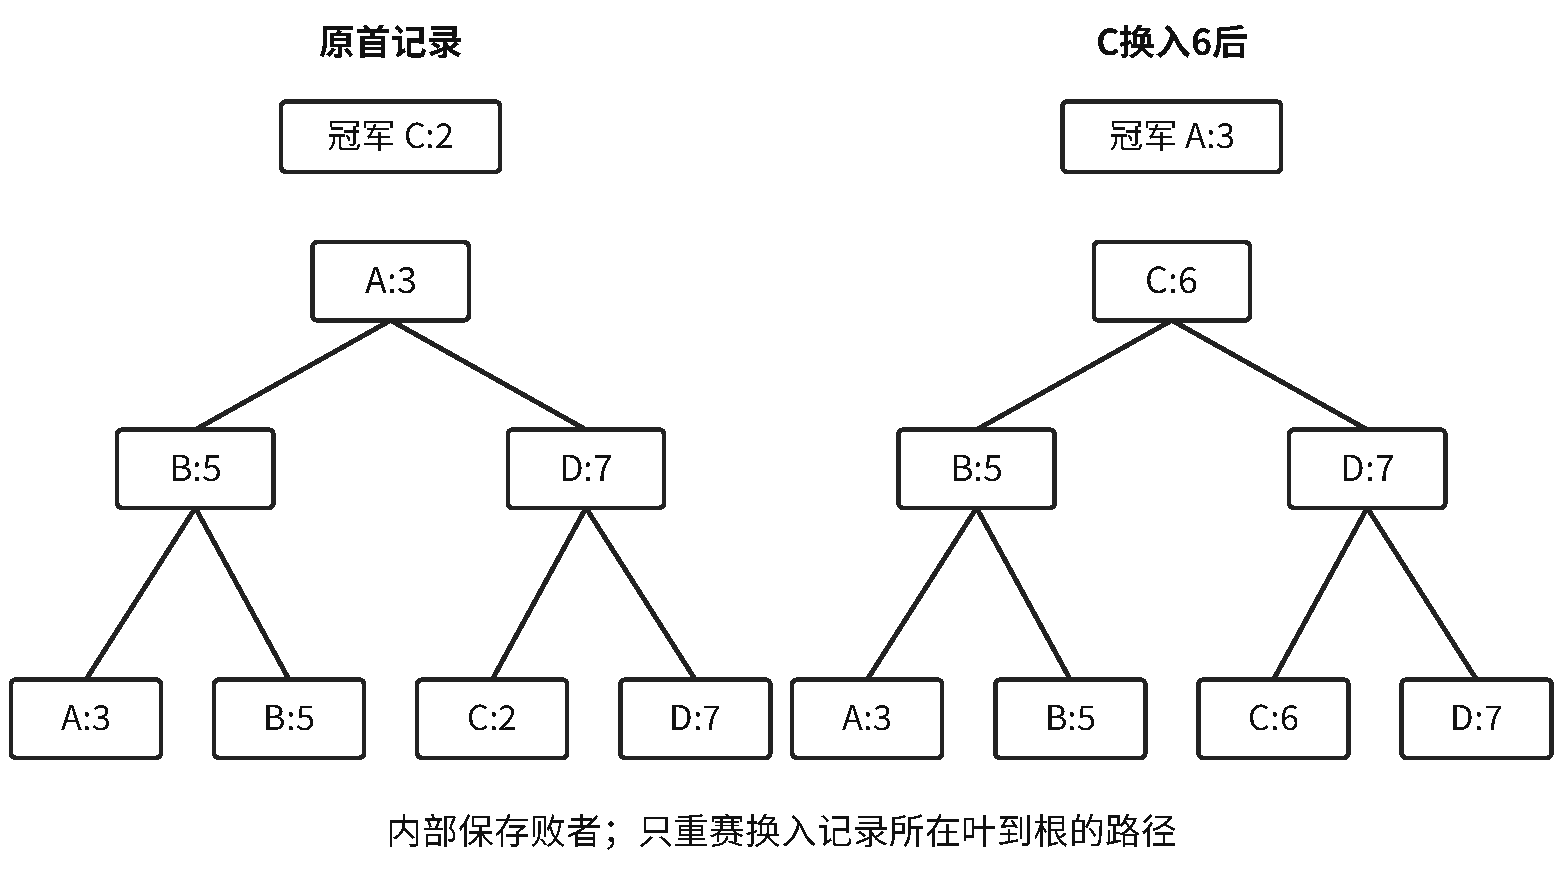
\includegraphics[width=\linewidth,height=108mm,keepaspectratio]{figures/DS_19_loser_tree.pdf}
\caption{内部保存败者，冠军单独记录}\label{DS08-loser-figure}
\end{figure}

不等长段的最佳归并以段长为叶权，最小化归并树WPL。二路每次合并当前两个最短段；\(k\)路每次合并当前\(k\)个最短段，先补最少零权叶，使\((r'-1)\bmod(k-1)=0\)。补虚段用于最优树的完整分支模型。

\par\medskip\Needspace{4\baselineskip}\noindent\hypertarget{DS08-E07}{}\label{DS08-E07}\textbf{例 8-8}\par\nobreak\smallskip

6个升序表A、B、C、D、E、F，分别含10、35、40、50、60、200个元素。通过5次两两合并成为一个升序表，要求最坏情况下比较总次数最小。

（1）给出完整合并过程及最坏比较总次数。（2）描述N个不等长升序表的合并策略并说明理由。

\par\medskip\Needspace{4\baselineskip}\noindent\hypertarget{DS08-E08}{}\label{DS08-E08}\textbf{例 8-9}\par\nobreak\smallskip

12个初始段长分别为30、44、8、6、3、20、60、18、9、62、68、85。进行4路外部归并，画出最佳归并树并计算WPL。

若段长以块计，每次归并完整读写，归并阶段I/O为\(2WPL\)，生成初始段另计；该口径按不等长段的各内部结点累计。

\section{排序性能与选择}\label{DS08-comparison}

下表为完整排序总时间。平均列比较排序采用互异关键字等概率排列；折半插入每趟完整定位，起泡有早停，归并无跳过有序段优化。

\par\smallskip
{\fontsize{9.3}{12}\selectfont\setlength{\tabcolsep}{2.5pt}\setlength{\LTleft}{0pt}\setlength{\LTright}{0pt}
\begin{longtable}{@{}>{\raggedright\arraybackslash}p{\dimexpr0.24500\linewidth-2\tabcolsep\relax}>{\raggedright\arraybackslash}p{\dimexpr0.26501\linewidth-2\tabcolsep\relax}>{\raggedright\arraybackslash}p{\dimexpr0.24500\linewidth-2\tabcolsep\relax}>{\raggedright\arraybackslash}p{\dimexpr0.24500\linewidth-2\tabcolsep\relax}@{}}
\toprule
算法 & 最好 & 平均 & 最坏 \\

\midrule\endfirsthead\toprule
算法 & 最好 & 平均 & 最坏 \\

\midrule\endhead\bottomrule\endfoot
直接插入 & \(\Theta(n)\) & \(\Theta(n^2)\) & \(\Theta(n^2)\) \\

折半插入 & \(\Theta(n\log n)\) & \(\Theta(n^2)\) & \(\Theta(n^2)\) \\

起泡 & \(\Theta(n)\) & \(\Theta(n^2)\) & \(\Theta(n^2)\) \\

简单选择 & \(\Theta(n^2)\) & \(\Theta(n^2)\) & \(\Theta(n^2)\) \\

希尔 & 依增量 & 依增量 & 依增量 \\

快速 & \(\Theta(n\log n)\) & \(\Theta(n\log n)\) & \(\Theta(n^2)\) \\

堆 & \(O(n\log n)\) & \(\Theta(n\log n)\) & \(\Theta(n\log n)\) \\

二路归并 & \(\Theta(n\log n)\) & \(\Theta(n\log n)\) & \(\Theta(n\log n)\) \\

LSD & \(\Theta(d(n+r))\) & 同左 & 同左 \\

计数 & \(\Theta(n+k)\) & 同左 & 同左 \\

\end{longtable}}
\par\smallskip

\par\smallskip
{\fontsize{9.3}{12}\selectfont\setlength{\tabcolsep}{2.5pt}\setlength{\LTleft}{0pt}\setlength{\LTright}{0pt}
\begin{longtable}{@{}>{\raggedright\arraybackslash}p{\dimexpr0.29737\linewidth-2\tabcolsep\relax}>{\raggedright\arraybackslash}p{\dimexpr0.33173\linewidth-2\tabcolsep\relax}>{\raggedright\arraybackslash}p{\dimexpr0.37089\linewidth-2\tabcolsep\relax}@{}}
\toprule
算法 & 辅助空间 & 稳定性条件 \\

\midrule\endfirsthead\toprule
算法 & 辅助空间 & 稳定性条件 \\

\midrule\endhead\bottomrule\endfoot
直接/折半插入 & \(O(1)\) & 相等新项放旧项后，稳定 \\

起泡 & \(O(1)\) & 仅严格逆序相邻交换，稳定 \\

简单选择、希尔、堆 & \(O(1)\) & 不稳定 \\

快速 & 栈平均\(O(\log n)\)、最坏\(O(n)\) & 不稳定 \\

归并 & \(\Theta(n)\) & 相等先取左段，稳定 \\

LSD & 链式\(O(r)\)；数组\(O(n+r)\) & 同桶保序，稳定 \\

计数 & \(\Theta(n+k)\) & 逆向按前缀和输出整记录，稳定 \\

\end{longtable}}
\par\smallskip

堆排序教材常在互异关键字模型把最好列为对数线性阶；允许全相等且下滤相等即停时，本章代码的建堆与输出可总计\(\Theta(n)\)。起泡无早停时，有序输入仍二次；归并若另加已有序段跳过判断，最好情况随之变化。

规模小或近有序可选直接插入；需最坏对数线性且常数空间可选堆；需稳定且可用线性辅助区可选归并；少量固定位、较小整数值域分别比较基数、计数代价。快排子区间、归并同层各段可独立处理；LSD各位有依赖，每位内部仍可设计并行分配。

仅靠两两比较区分\(n\)个互异关键字全部排列时，决策树至少有\(n!\)叶，最坏比较次数至少\(\lceil\log_2(n!)\rceil=\Omega(n\log n)\)。计数、基数利用关键字值域或数位结构，适用另一成本模型。
